%!TEX root = ../../main.tex

\chapter{Aktueller Stand und Analyse der CO2-Runter-App}
\label{chapter:2}

Im Rahmen dieser Studienarbeit steht die Erfassung des aktuellen Zustands und die Analyse der CO2-Runter App im Fokus. Dies ist insbesondere wichtig, um vor Beginn unserer eigentlichen Arbeit eine umfassende Bestandsaufnahme vorzunehmen und die bestehenden Probleme zu identifizieren. Zunächst vorweg sollte geklärt werden, dass häufiger der Begriff \textit{App} fallen wird. Dies soll nicht bedeuten, dass es sich hierbei um eine mobile Applikatin (App) handelt. Eigentlich ist es nämlich eine Webseite und im Verlaufe dieser Studienarbeit wird App und Webseite teilweise synonym verwendet. Die Startseite der CO2-Runter App dient als Einstiegspunkt für alle Nutzer. Die Startseite spielt eine entscheidende Rolle, da sie den ersten Eindruck vermittelt und die Nutzer dazu anregen sollte, sich weiter mit der App zu beschäftigen. Da das Hauptziel der App darin besteht, die Nutzer dazu zu bewegen, ihren persönlichen CO2-Fußabdruck zu ermitteln, ist es von besonderer Bedeutung, dass die Webseite die Nutzer aktiv dazu motiviert, diese Aufgabe anzugehen. Die Abbildung \ref{fig:co2runterapp-landingpage} zeigt die Startseite der Webseite\footnote{Die Startseite ist unter folgendem Link erreichbar: https://co2runter.karlsruhe.de/ \cite{co2runterapp}}. Bei einem ersten Blick auf die Webseite fallen mehrere Unstimmigkeiten auf. Die Dropdown-Felder wirken unverhältnismäßig lang und stören die Proportionen des Layouts. Die Webseite selbst erscheint unstrukturiert und wenig organisiert, was zu einer geringen Benutzerfreundlichkeit führt. Besonders auffällig ist der Mangel an klaren Handlungsanweisungen, die den Nutzer zur Interaktion und aktiven Nutzung der App ermutigen sollen.

\begin{figure}[h]
    \centering
    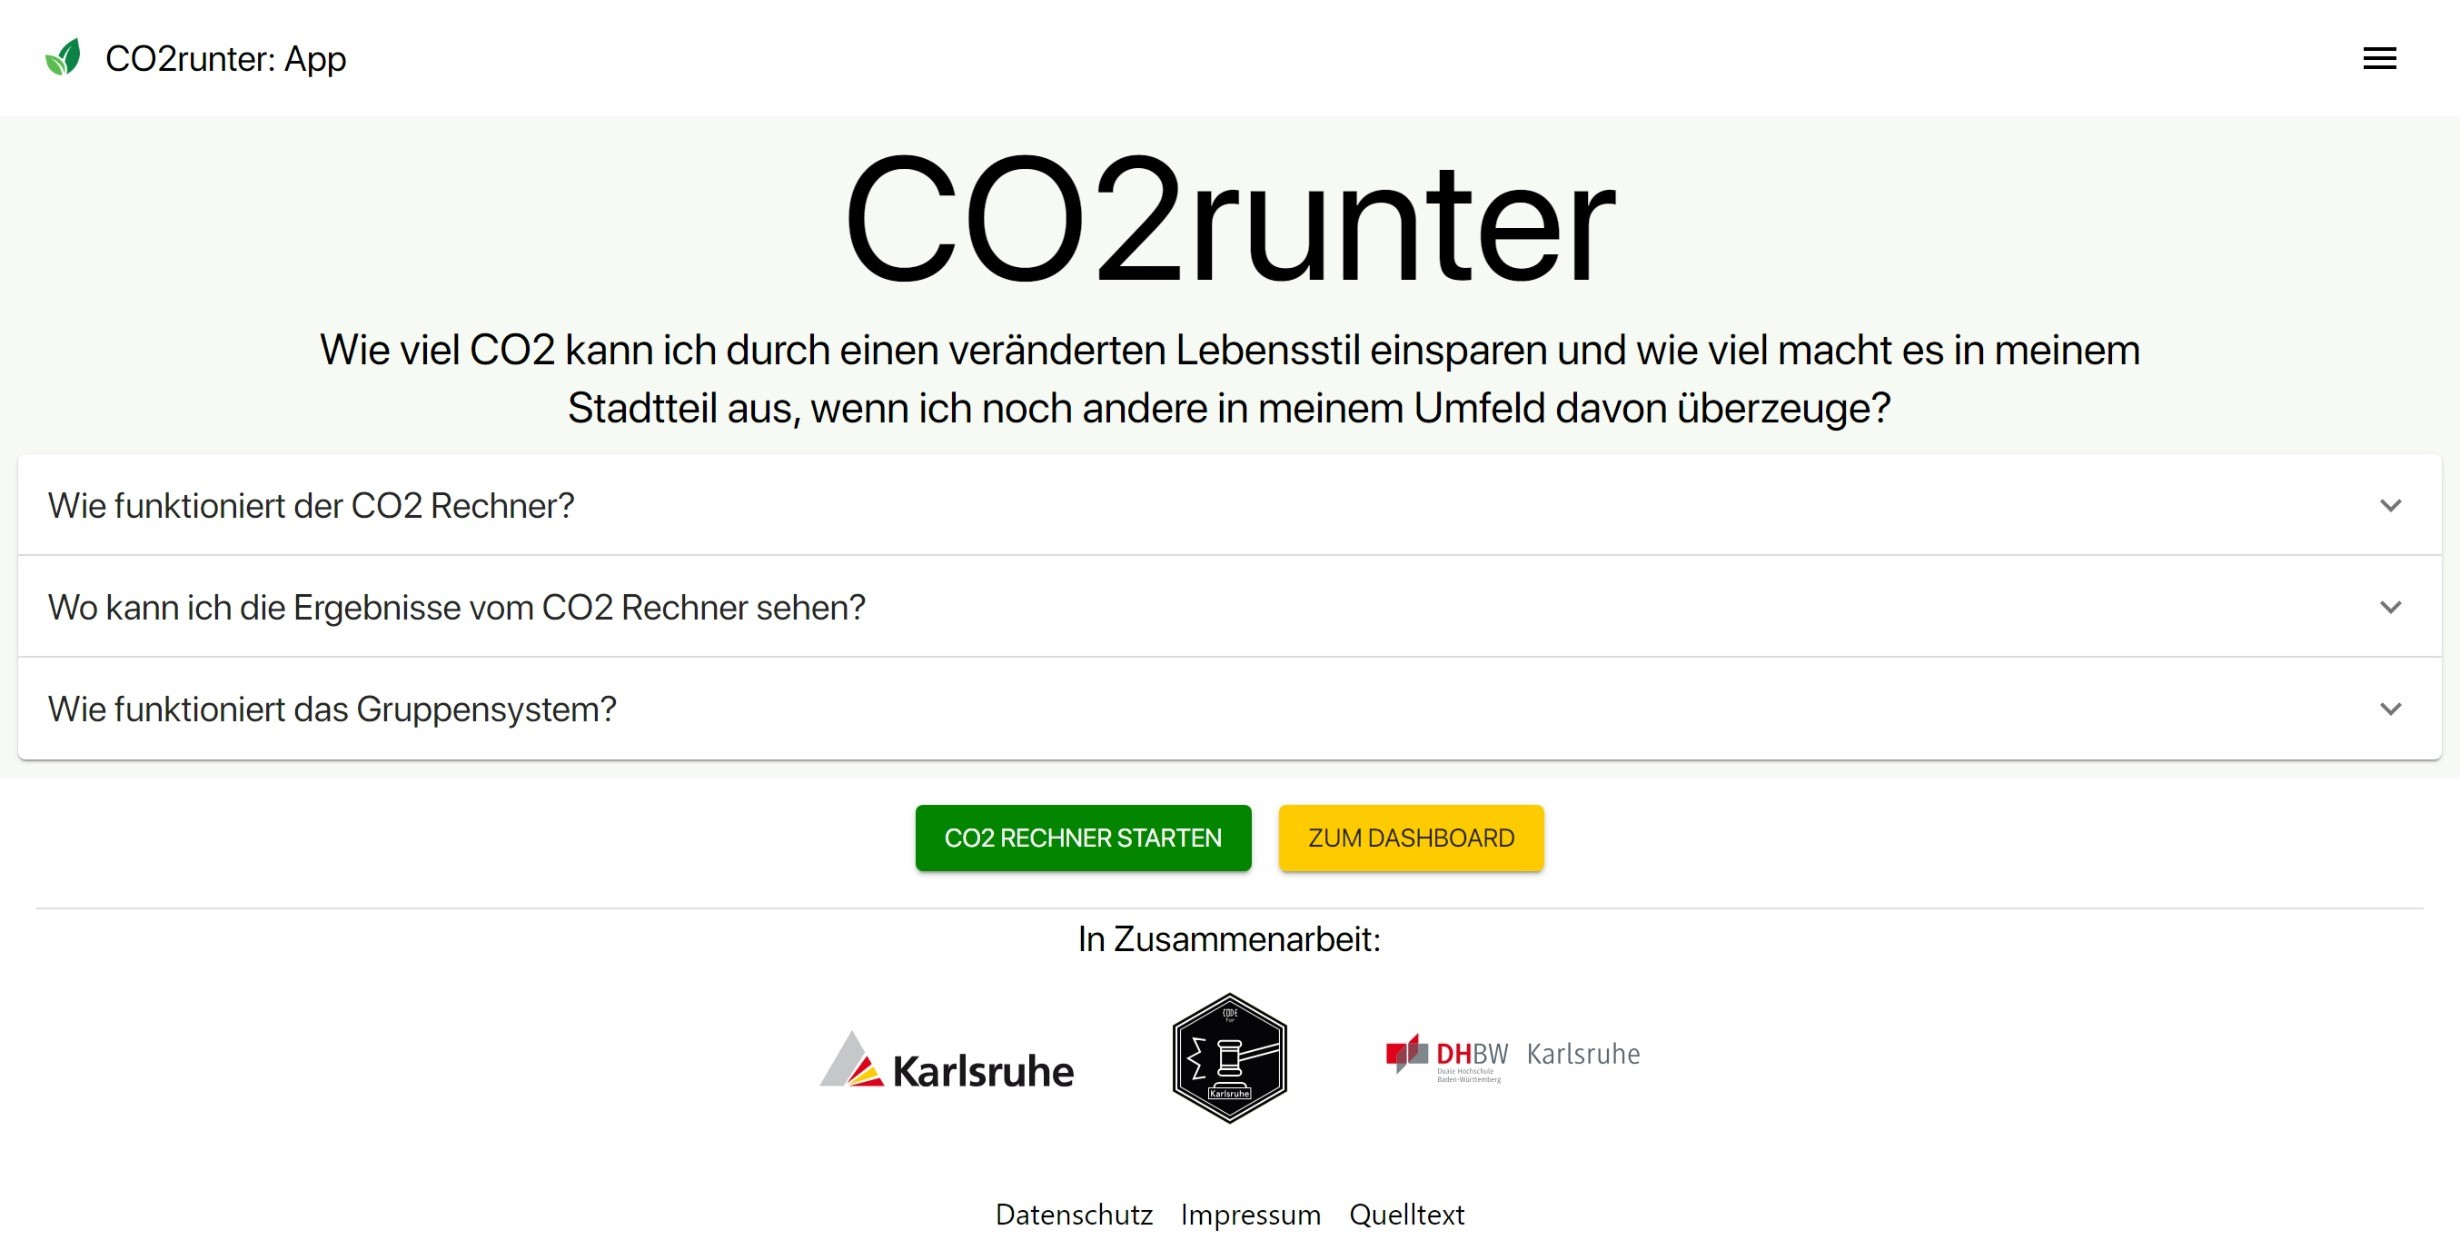
\includegraphics[width=0.7\textwidth]{images/02/CO2-Runter-App-Landingpage.jpeg}
    \caption{Startseite der CO2-Runter-App}
    \label{fig:co2runterapp-landingpage}
\end{figure}

Erst nach längerem Verweilen auf der Seite werden die Buttons \texttt{CO2 Rechner Starten} und \texttt{zum Dashboard} sichtbar. Dennoch bleibt unklar, was sich hinter dem Begriff \texttt{Dashboard} verbirgt und warum es für den Nutzer von Interesse sein sollte. Es fehlt eine klare Aufforderung, den Nutzer zur aktiven Teilnahme zu bewegen und ihn dazu zu inspirieren, sich eingehender mit der Webseite zu beschäftigen.

Die ideale Startseite sollte dem Besucher eine übersichtliche und strukturierte Präsentation bieten und ihn unmittelbar dazu motivieren, seinen persönlichen CO2-Fußabdruck zu ermitteln oder die Daten der Karlsruher Stadtteile zu sehen.

Wenn der Nutzer sich dazu entscheidet, den Button \texttt{CO2 Rechner Starten} zu betätigen, wird er auf eine Seite weitergeleitet, die in Abbildung \ref{fig:co2runterapp-rechner} dargestellt ist.

\begin{figure}[h]
    \centering
    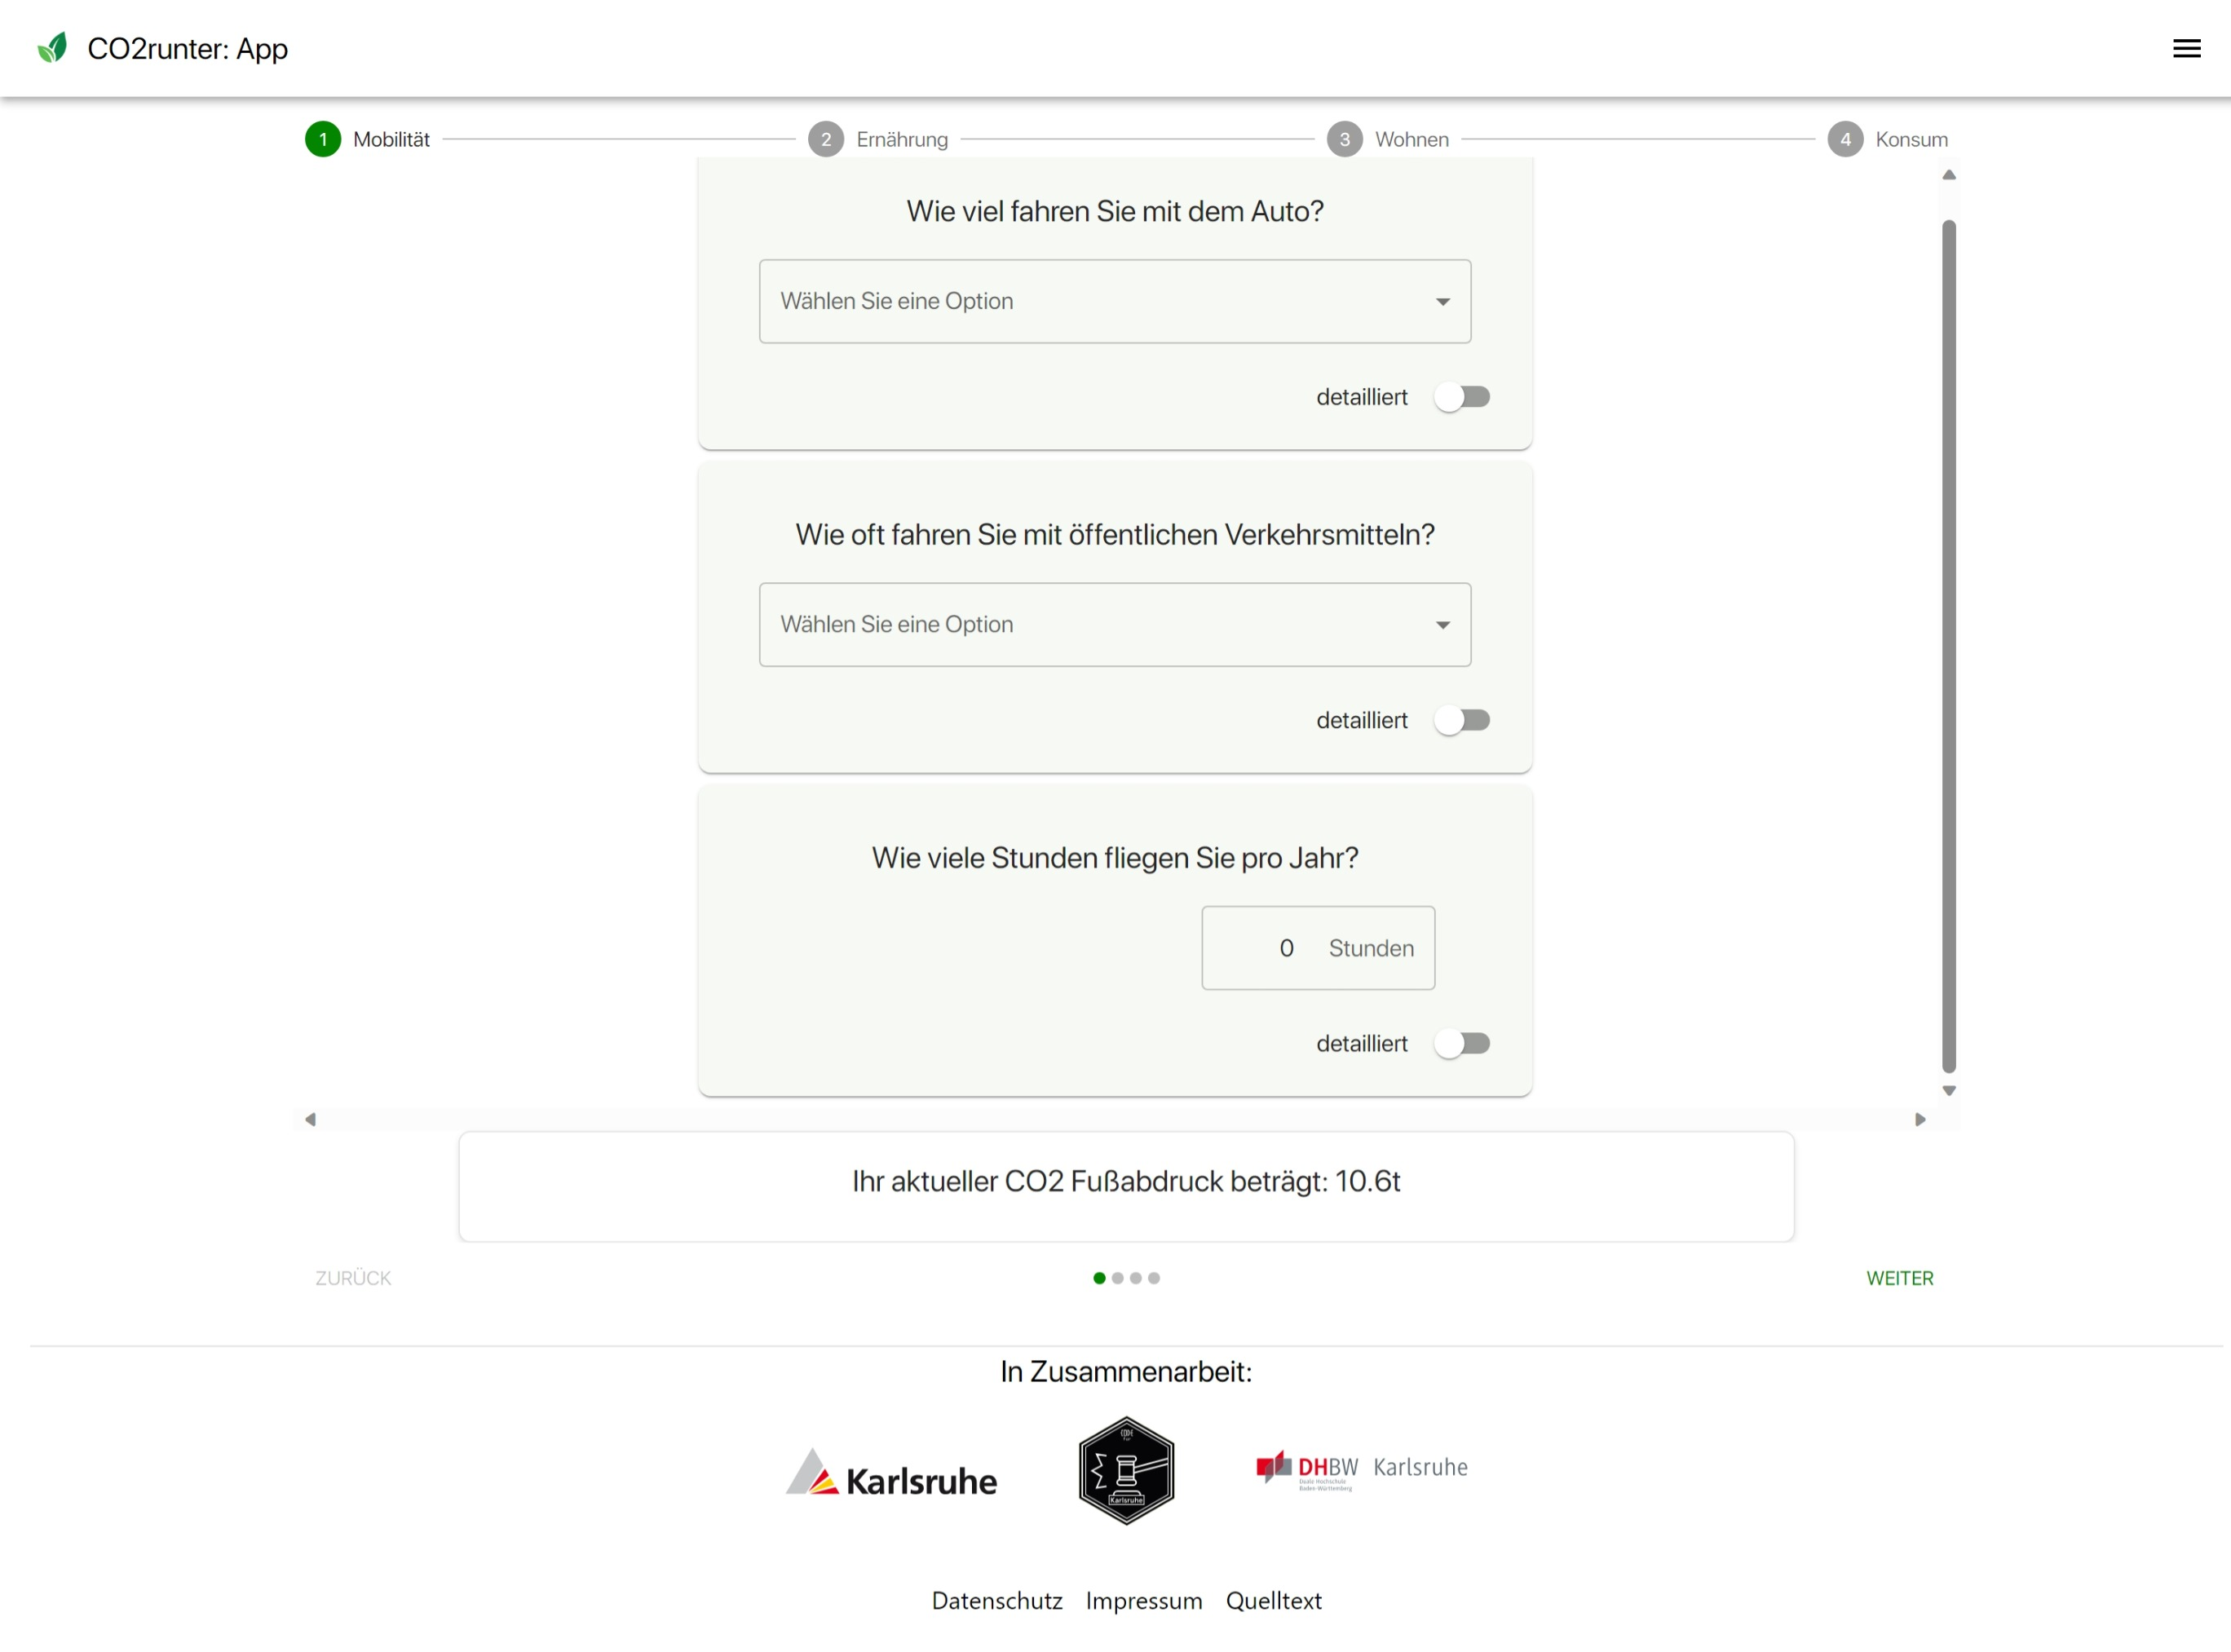
\includegraphics[width=1\textwidth]{images/02/CO2-Runter-App-Rechner.jpeg}
    \caption{CO2 Rechner Formular der CO2A Runter App}
    \label{fig:co2runterapp-rechner}
\end{figure}

Auf dieser Seite wird dem Nutzer ein Formular präsentiert, das er ausfüllen muss, um seinen endgültigen CO2-Fußabdruck zu bestimmen. Anschließend kann er diese Daten einem Stadtteil von Karlsruhe zuordnen und versenden oder ohne Datenübertragung fortfahren, was ihn direkt zum Dashboard führt. Die Möglichkeit, diese Entscheidung zu treffen, wird in Abbildung \ref{fig:co2runterapp-send} illustriert. (Siehe nächste Seite)

\begin{figure}[h]
    \centering
    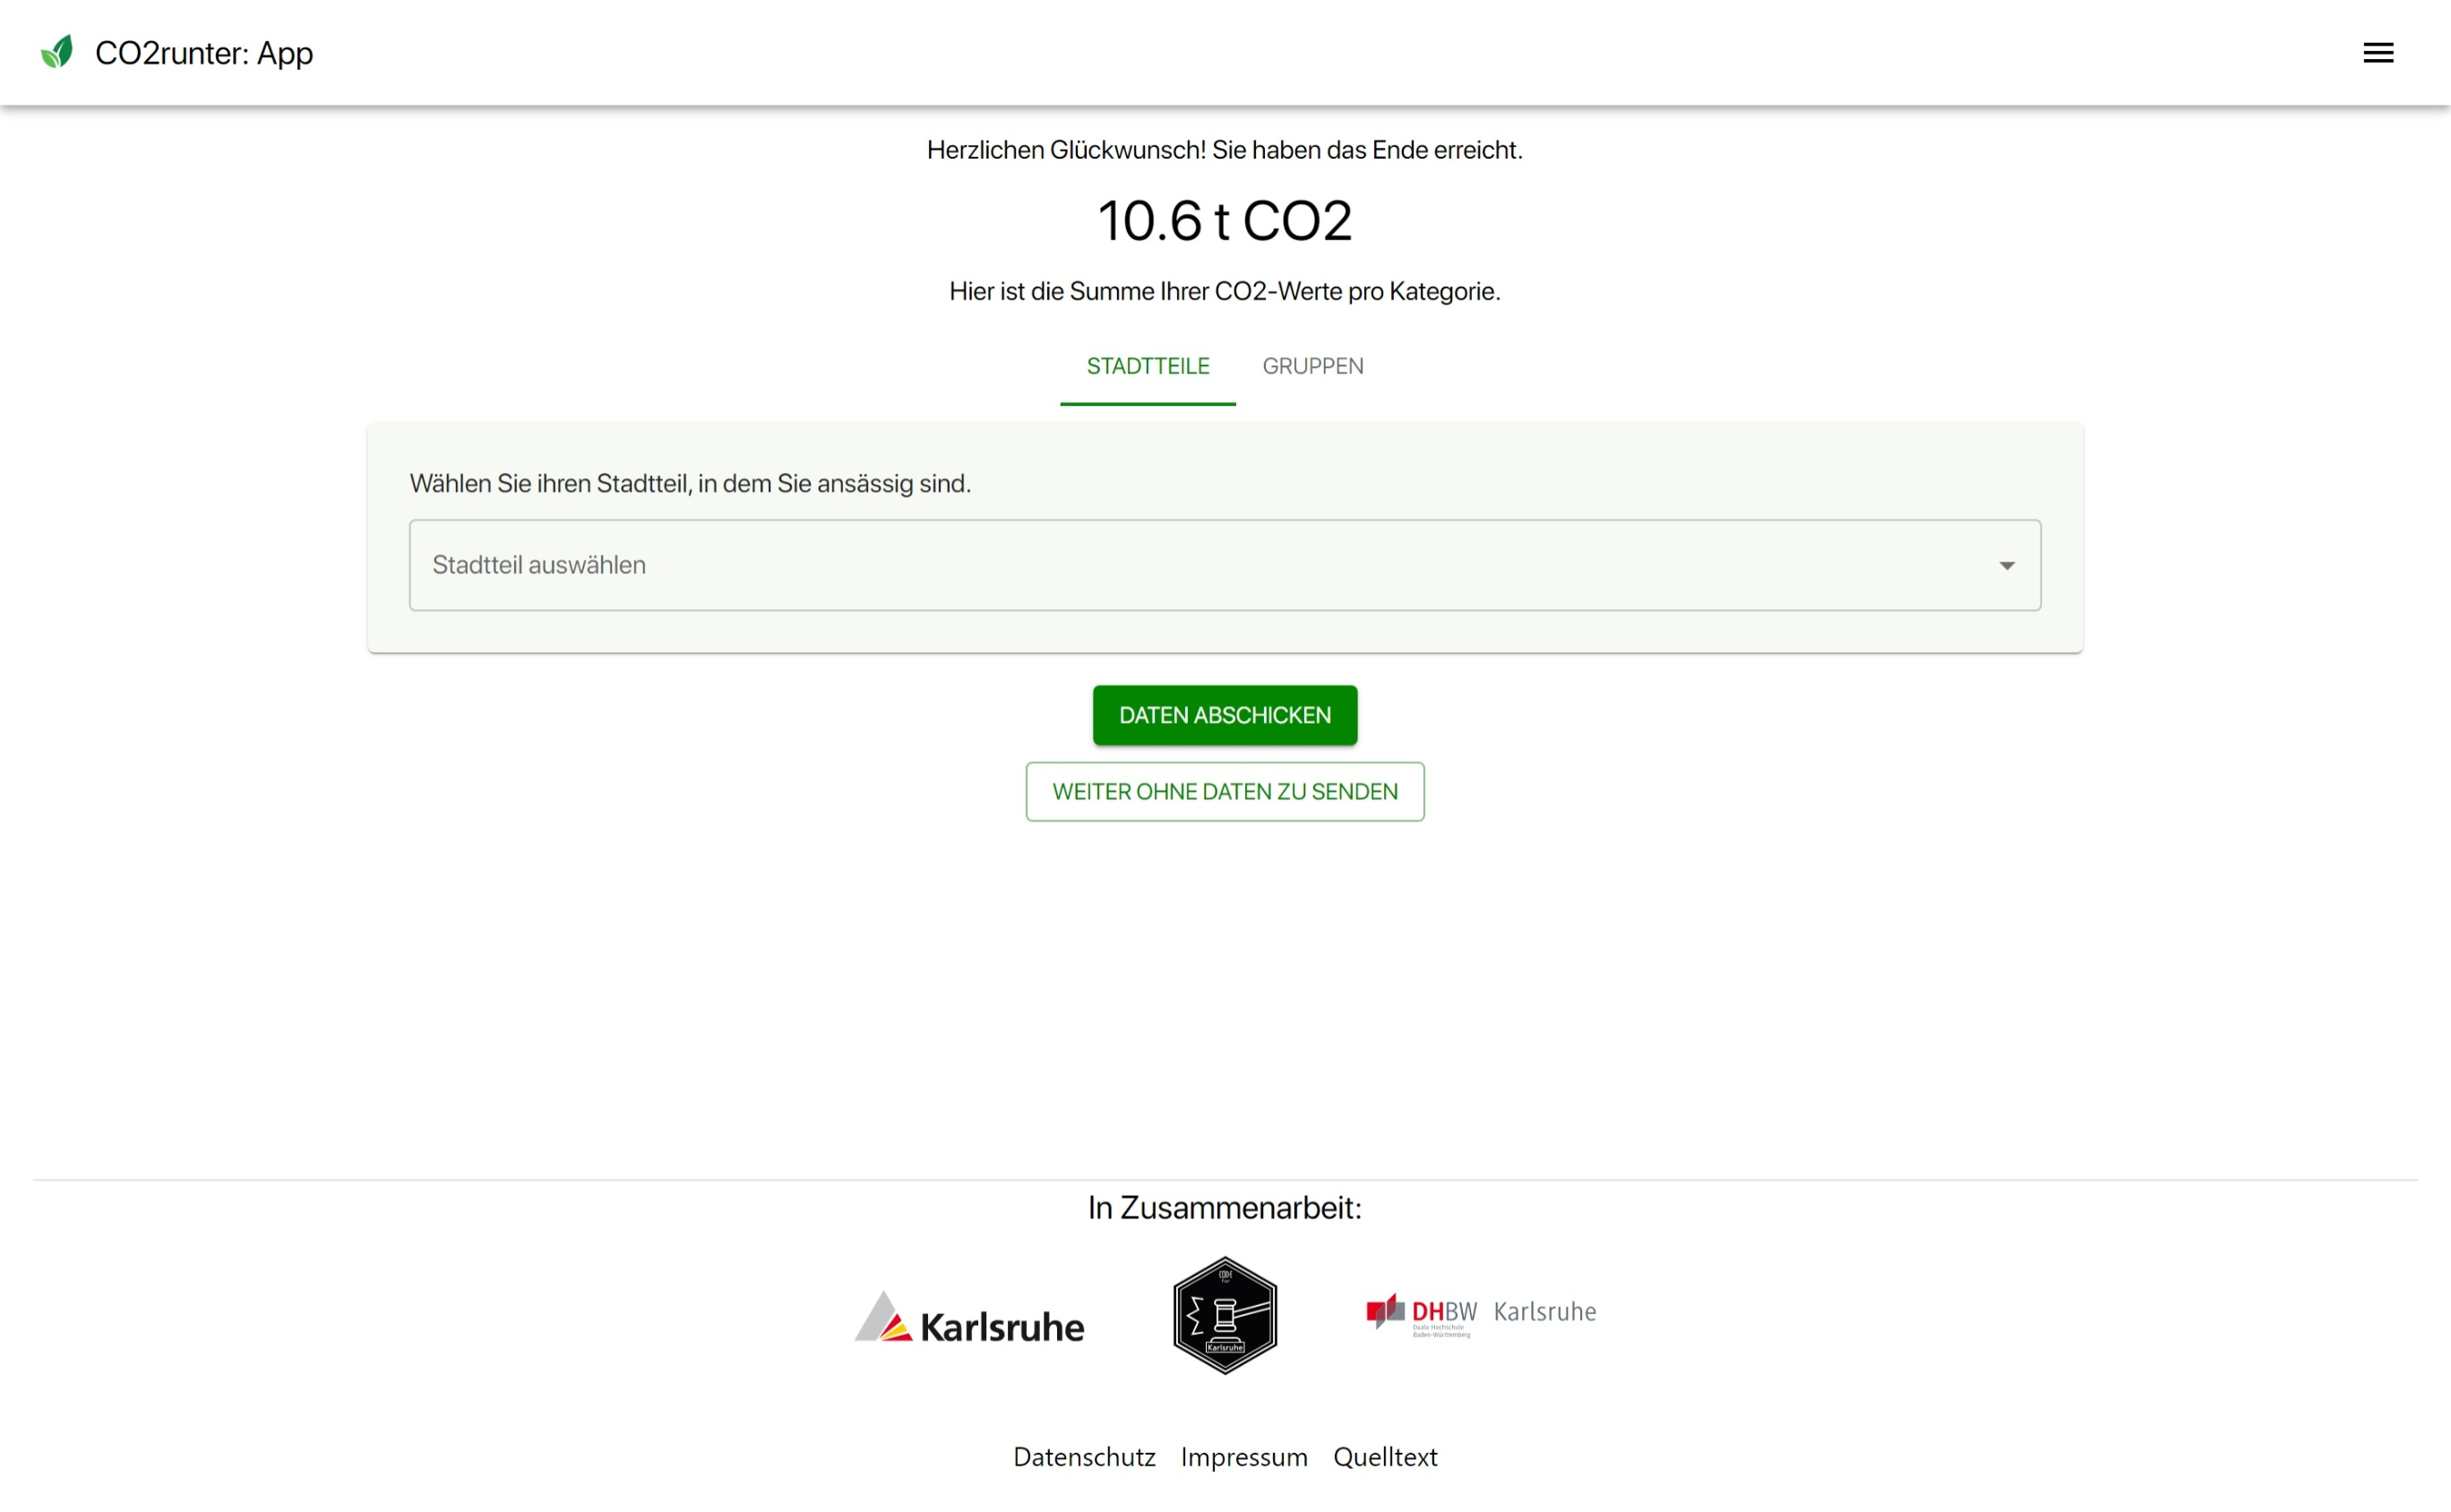
\includegraphics[width=1\textwidth]{images/02/CO2-Runter-App-Daten-Senden.jpeg}
    \caption{CO2 Rechner Formular Daten senden der CO2A Runter App}
    \label{fig:co2runterapp-send}
\end{figure}

Die letzte Hauptfunktion ist das Dashboard, das die übermittelten Nutzerdaten in Grafiken anzeigt. In der Kartengrafik werden die CO2-Emissionen der Stadtteile von Karlsruhe dargestellt. Diese kommen zustande, indem Nutzer beim Berechnen ihrer CO2-Bilanz angeben, aus welchem Stadtteil sie aus Karlsruhe kommen, wodurch sich diese Daten anpassen können. Neben der Karten-Grafik gibt es noch die Charts, in denen der durchschnittliche Betrag folgenden Kategorien zugewiesen werden kann: Mobilität, Wohnen, Konsum, Ernährung und Infrastruktur. Im Gruppen-Tab sieht man wiederum, welche Gruppe wie viel CO2 verbraucht hat, und im letzten Tab, wie der Name schon verrät, wird ein Balkendiagramm angezeigt, welches die Beteiligung der Nutzer und in welchem Stadtteil diese wohnen. Die Abbildung \ref{fig:co2runterapp-dashboard} zeigt die Kartengrafik des Dashboards und die jeweilige Menge an CO2, die den Stadtteilen zugeordnet wurden.

\newpage

\begin{figure}[h]
    \centering
    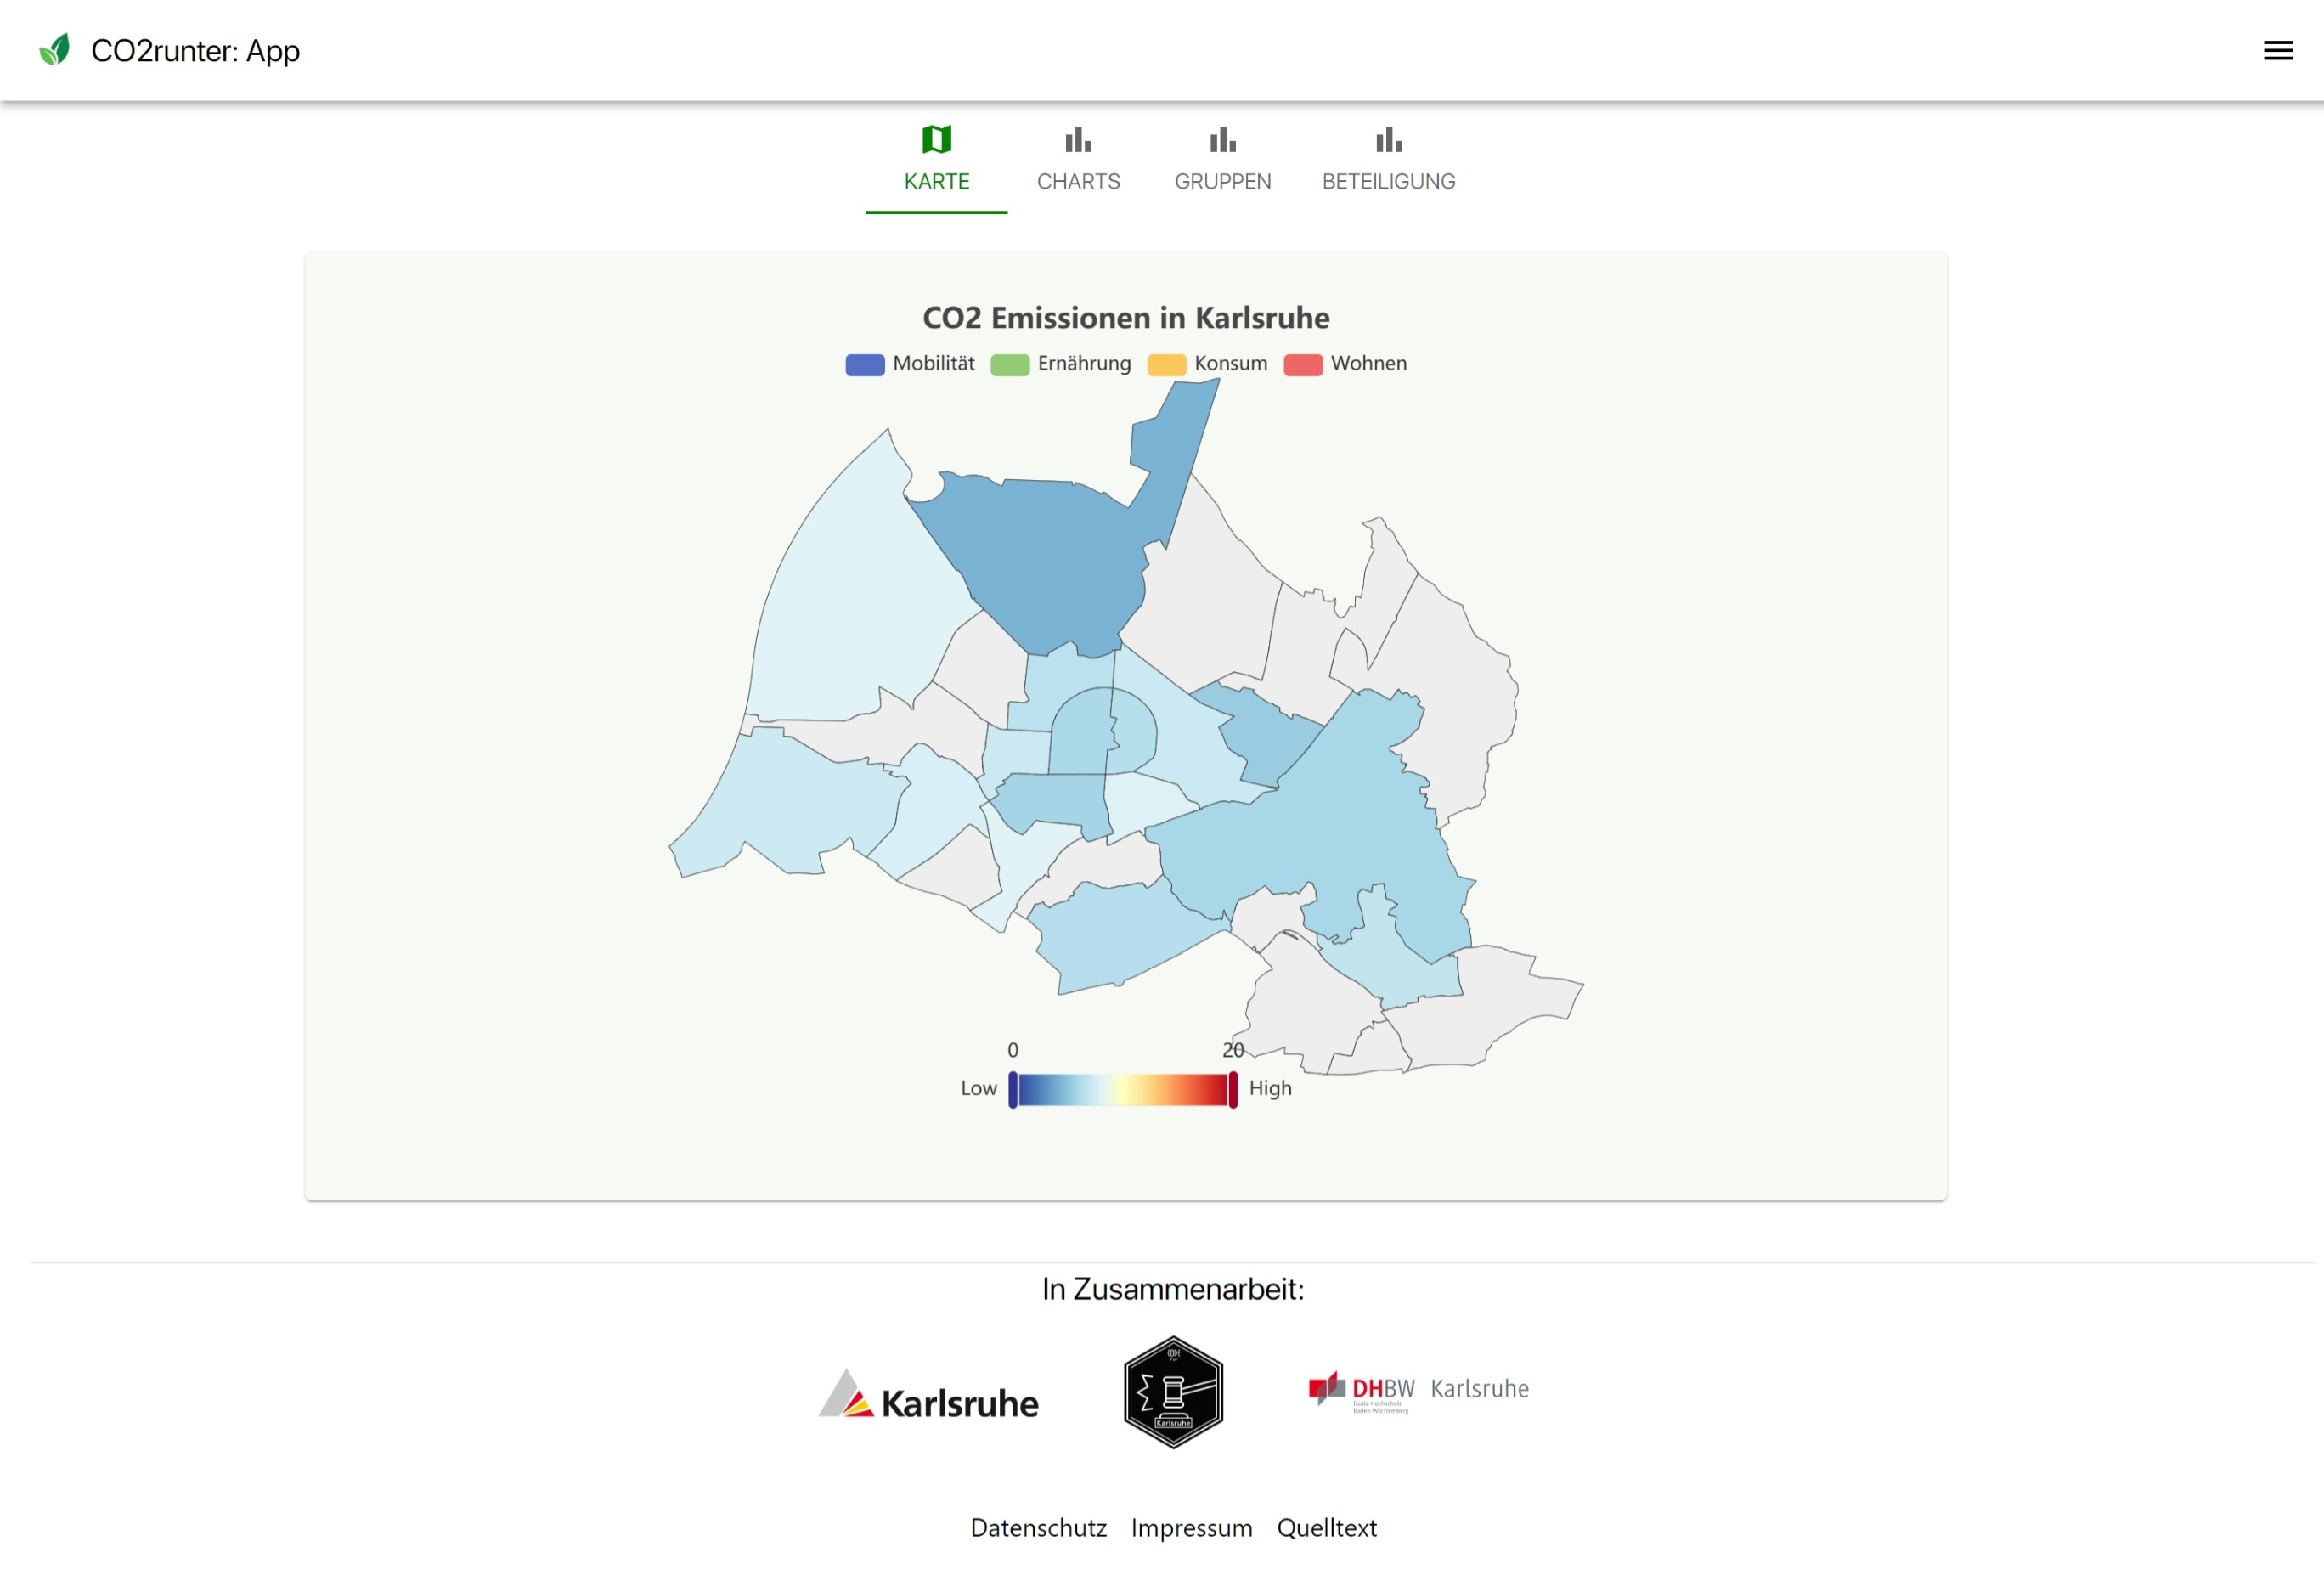
\includegraphics[width=1\textwidth]{images/02/CO2-Runter-App-Dashboard.jpeg}
    \caption{CO2 Dashboard der CO2A Runter App}
    \label{fig:co2runterapp-dashboard}
\end{figure}

Insgesamt bietet die CO2-Runter App eine Plattform zur Berechnung und Vergleich des CO2-Fußabdrucks, wobei der Fokus auf einer verbesserten Benutzerfreundlichkeit und klaren Handlungsanweisungen liegen sollte, um die aktive Beteiligung der Nutzer zu fördern.
Die Struktur und Anordnungen der Unterseiten sehen im Vergleich zur Startseite wesentlich strukturierter und organisierter aus, und als Nutzer weiß man eher, was zu tun ist.
